\documentclass{article}

% Page margin
\usepackage[margin=1in,includefoot]{geometry}

% Header and Footer
\usepackage{fancyhdr}
\pagestyle{fancy}
\fancyfoot{}
\fancyfoot[R]{page \thepage}

% Graphics preamble
\usepackage{graphicx}
\usepackage{float}

% Text Symbols
\usepackage{textcomp}

\begin{document}
\begin{titlepage}
\title{\bfseries Measurement of Hydrocarbon Level in Urban Setting \\
	\large CE344}
\author{Donghyeon Kim}
\date{November 16, 2017}
\maketitle
\thispagestyle{empty}
\end{titlepage}

% Abstract
\begin{abstract}
Hydrocarbon level is a good indicator of pollution within urban context. In this experiment, we conducted three different forms of hydrocarbon measurements in New York, New York. In the first part of the experiment, hydrocarbon within the air near the major roadways was measured to estimate the influence of vehicular traffic to air pollution. In the second part of the experiment, chlorinated hydrocarbon within soil samples was measured qualitatively to estimate the amount of insecticides and other toxic chemicals in soils. In the third part of the experiment, total hydrocarbon within soil samples was measured. Overall contamination level was high and health of urban residents are of concern.
\end{abstract}

% Table of Contents
\tableofcontents
\listoffigures
\listoftables
\thispagestyle{empty}
\newpage

\setcounter{page}{1}
\section{Procedure}\label{sec:procedure}

See the attached instructions for each part of the experiment.

\section{Result}\label{sec:result}
\subsection{Part 1}

\begin{table}[h!]
	\begin{center}
		\begin{tabular}{c|rrrr}
			\textbf{ID} & \textbf{Methane (ppm)} & \textbf{Temperature (\textcelsius)} & \textbf{Wind Speed (m/s)} & \textbf{Traffic (cars/min)} \\ \hline
			1 & 90 & 27.8 & 1.5 & 26 \\
			2 & 57 & 28.8 & 0.8 & 20 \\
			3 & 58 & 27.6 & 1.6 & 24 \\
			4 & 68 & 29.2 & 1.6 & 21 \\
			5 & 60 & 28.3 & 2.0 & 23 \\
			6 & 28 & 29.3 & 0.6 & 18 \\
			7 & 44 & 28.4 & 0.7 & 19 \\
			8 & 40 & 28.6 & 0.8 & 20 \\
			9 & 34 & 29.5 & 0.7 & 21 \\
			10 & 28 & 29.7 & 0.7 & 21 \\
			11 & 48 & 27.8 & 0.4 & 22 \\
			12 & 48 & 28.6 & 1.0 & 21 \\
			13 & 47 & 28.4 & 1.6 & 17 \\
			14 & 48 & 28.8 & 1.1 & 9\\
		\end{tabular}
		\caption[Part 1 Result]{Result of part 1 of this experiment is shown.}
		\label{tab:part1}
	\end{center}
\end{table}

The result of measurements conducted by 4 subgroups is compiled in Table \ref{tab:part1}. To observe the relation between independent variables, methane concentration was plotted against each variables and best fit power curve was calculated.

\begin{figure}[h!]
	\centering
	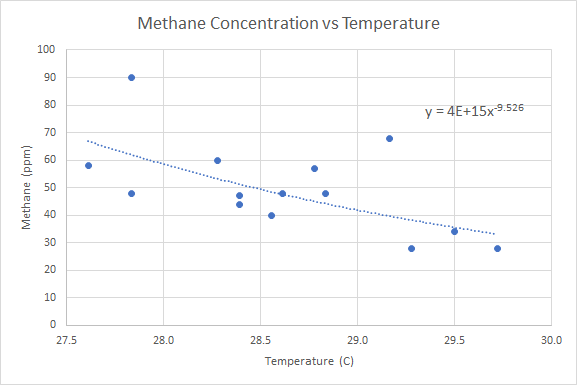
\includegraphics[width=0.7\linewidth]{part1_temp}
	\caption[Methane vs Temperature]{Methane (ppm) vs Temperature (\textcelsius). $y = 4E+15x^{-9.526}$}
	\label{fig:part1temp}
\end{figure}

\begin{figure}[h!]
	\centering
	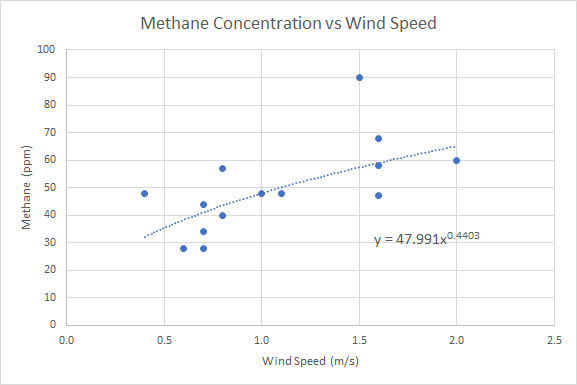
\includegraphics[width=0.7\linewidth]{part1_wind}
	\caption[Methane vs Wind Speed]{Methane (ppm) vs Wind Speed (m/s). $y = 47.991x^{0.4403}$}
	\label{fig:part1wind}
\end{figure}

\begin{figure}[h!]
	\centering
	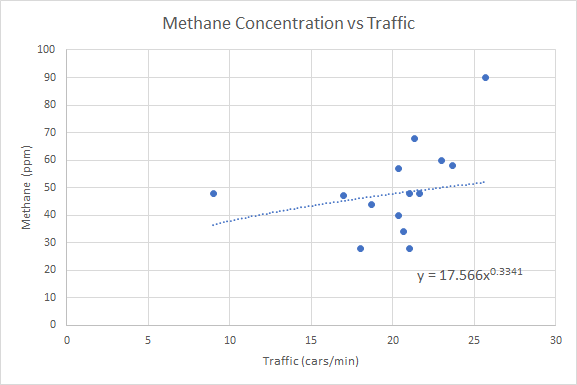
\includegraphics[width=0.7\linewidth]{part1_traffic}
	\caption[Methane vs Traffic]{Methane (ppm) vs Traffic (cars/min). $y = 17.566x^{0.3341}$}
	\label{fig:part1traffic}
\end{figure}

Amount of traffic was not strongly correlated to methane concentration in air, while temperature had negative correlation and wind speed had positive correlation. Empirical formula we came up with our data is the following:

\begin{equation} \label{eq:empirical}
C = 2 \times 10^{16} \times T^{-10} V^{0.5}
\end{equation}

where

$C = Methane\ Concentration\ (ppm)$

$T = Temperature$ (\textcelsius)

$V = Wind\ Speed\ (m/s)$

\subsection{Part 2}

\begin{table}[h!]
	\begin{center}
		\begin{tabular}{c|rrr}
			\textbf{ID} & \parbox{4.8cm}{\textbf{Chlorinated Hydrocarbon (ppm)}} & \textbf{DF} & \textbf{Actual (ppm)} \\ \hline 
			1 & HIGH & 1.00 & HIGH \\
			2 & HIGH & 1.00 & HIGH \\
			3 & HIGH & 1.00 & HIGH \\
			4 & 27.5 & 1.00 & 27.5 \\
			5 & 25.0 & 1.00 & 25.0 \\
			6 & 35.0 & 1.00 & 35.0 \\
			7 & 5.0 & 1.00 & 5.0 \\
			8 & 25.0 & 1.00 & 25.0 \\
			9 & 40.0 & 1.00 & 40.0 \\
			10 & 45.0 & 2.00 & HIGH \\
			11 & 25.0 & 1.01 & 25.3 \\
			12 & HIGH & 1.00 & HIGH \\
			13 & 25.0 & 0.90 & 22.5 \\
			14 & 23.0 & 1.00 & 23.0 \\
			15 & 32.0 & 1.00 & 32.0 \\
			16 & HIGH & 1.00 & HIGH \\
			17 & 25.0 & 1.00 & 25.0 \\
			18 & 35.0 & 1.00 & 35.0 \\
			19 & 45.0 & 1.00 & 45.0 \\
			20 & 25.0 & 1.00 & 25.0 \\			
		\end{tabular}
		\caption[Part 2 Result]{Result of part 2 of this experiment is shown. Readings that exceeded 50ppm is shown as HIGH. Actual concentration is calculated by multiplying actual reading by dilution factor(DF).}
		\label{tab:part2}
	\end{center}
\end{table}

Readings of chlorinated hydrocarbon in soil samples taken from surface of New York City are show in Table \ref{tab:part2}. Actual concentration of chlorinated hydrocarbon is then calculated with dilution factor of each samples. In this experiment, response factor(RF) was not used.

\begin{figure}[h!]
	\centering
	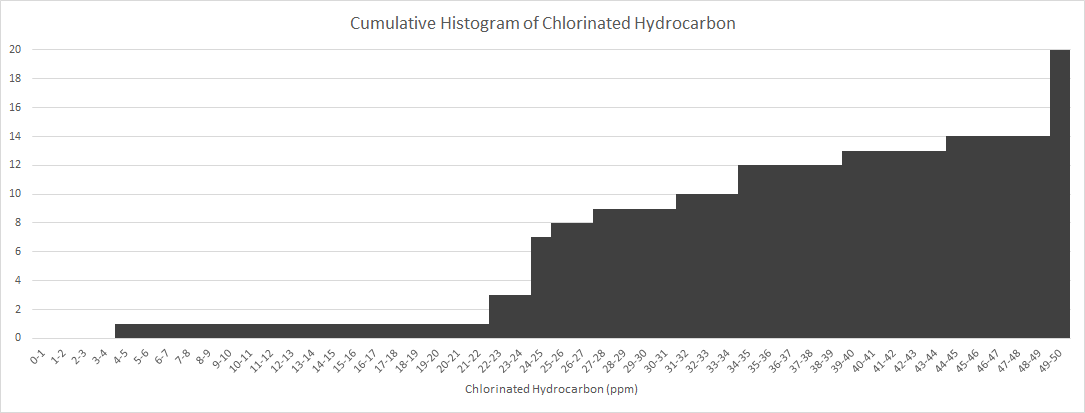
\includegraphics[width=1\linewidth]{part2}
	\caption[Part 2 Summary]{Cumulative histogram of chlorinated hydrocarbon measured in each soil sample.}
	\label{fig:part2sum}
\end{figure}

\begin{table}[h!]
	\begin{center}
		\begin{tabular}{r|c}
			Total Number of Samples & 20 \\
			Number of Samples $>$50ppm & 6 \\ \hline
			\% of Samples $>$50ppm & 30 \\
		\end{tabular}
		\caption[Part 1 Summary]{Summary of part 2 of this experiment.}
		\label{tab:part2sum}
	\end{center}
\end{table}

Actual concentration of chlorinated hydrocarbon in Table \ref{tab:part2} is plotted in Figure \ref{fig:part2sum} as a cumulative histogram. Samples that had chlorinated hydrocarbon concentration higher than 50ppm was 30 percent of all samples as shown in Table \ref{tab:part2sum}.

\subsection{Part 3}

\begin{table}[h!]
	\begin{center}
		\begin{tabular}{c|c|rr}
			\textbf{Group} & \textbf{ID} & \textbf{Weight (g)} & \textbf{Hydrocarbon (ppm)} \\ \hline
			A & 1 & 10.0 & 1185 \\
			A & 2 & 10.8 & 977 \\
			A & 3 & 10.0 & 1572 \\
			A & 4 & 10.0 & 2017 \\
			A & 5 & 10.0 & 1283 \\
			A & 6 & 10.0 & 848 \\
			A & 7 & 10.0 & 3216 \\
			A & 8 & 10.0 & 187 \\
			A & 9 & 10.0 & 396 \\
			A & 10 & 10.0 & 253 \\
			A & 11 & 10.3 & 1416 \\
			A & 12 & 10.0 & 1281 \\
			A & 13 & 10.1 & 822 \\
			A & 14 & 10.0 & 719 \\
			A & 15 & 10.0 & 1064 \\
			A & 16 & 10.0 & 1585 \\
			A & 17 & 8.7 & 2222 \\
			A & 18 & 10.0 & 1194 \\
			A & 19 & 10.1 & 1347 \\
			A & 20 & 10.0 & 1292 \\
			A & 21 & 10.0 & 684 \\ \hline
			B & 1 & 10.0 & 2302 \\
			B & 2 & 9.8 & 287 \\
			B & 3 & 9.9 & 1405 \\
			B & 4 & 10.1 & 1478 \\
			B & 5 & 9.9 & HIGH \\
			B & 6 & 10.0 & 844 \\
			B & 7 & 10.0 & 2058 \\
			B & 8 & 10.2 & 360 \\
			B & 9 & 10.0 & 1079 \\
			B & 10 & 10.1 & 2728 \\
			B & 11 & 10.2 & 2362 \\
			B & 12 & 10.0 & 896 \\
			B & 13 & 9.8 & HIGH \\
			B & 14 & 10.0 & 874 \\
			B & 15 & 10.0 & 726 \\
			B & 16 & 10.1 & 1702 \\
			B & 17 & 10.0 & 183 \\
			B & 18 & 9.8 & 2230 \\
			B & 19 & 10.2 & 2310 \\
			B & 20 & 10.1 & 1088 \\
			B & 21 & 10.0 & 2088 \\ \hline \hline
			\multicolumn{3}{r}{\textbf{Average}} & 1314 \\
			\multicolumn{3}{r}{\textbf{Standard Deviation}} & 739 \\
		\end{tabular}
		\caption[Part 3 Result]{Result of part 3 of this experiment is shown. Readings greater than the upper bound of the measuring device are shown as HIGH.}
		\label{tab:part3}
	\end{center}
\end{table}

According to Table \ref{tab:part3}, average hydrocarbon concentration of soil samples was 1314 ppm and standard deviation was 739 ppm. 2 soil samples had higher hydrocarbon concentration than the upper bound of measurable range, and excluded from final analysis.

\section{Discussion}\label{sec:discussion}
\subsection{Part 1}

Although we first expected the amount of traffic on adjacent road would have greatest influence on methane concentration in air, air temperature had the strongest correlation to methane concentration (power of -10, Figure \ref{fig:part1temp}). Wind speed had positive correlation to methane concentration (power of 0.5, Figure \ref{fig:part1wind}), but significantly small compared to temperature's influence. From Equation \ref{eq:empirical}, we can expect higher methane concentration during summer than during winter. Also, areas near water body (i.e. river, lake, ocean) will have lower methane concentration during summer than areas that have a lot of asphalt roads and concrete buildings where atmosphere heats up faster.

\subsection{Part 2}

As shown in Table \ref{tab:part2sum}, 30\% of total sample exceeded 50ppm chlorinated hydrocarbon concentration, which is unsafe for citizens that are exposed to the soil. Also, most of soil samples had concentration higher than 22 ppm according to Figure \ref{fig:part2sum}. Many of soil samples tested in this experiment were excavated from public parks and playgrounds of New York City, therefore, younger population whose daytime activity involve direct contact to the polluted soil are under health risk.

Since most of chlorinated hydrocarbon in municipal environment originates from insecticides and herbicides applied to soil, reduction of chlorine-based product is recommended in order to reduce the chlorinated hydrocarbon concentration in New York City's soil. Frequent monitoring of municipal soil is needed for contaminated sites, because qualitative analysis of soil, like the one conducted in this experiment, can be achieved in large quantity within short time frame.

\subsection{Part 3}

Kansas Department of Health and Environment limits TPH (total petroleum hydrocarbon) in soil up to 550 ppm for residential uses, and 950 ppm for non-residential uses, because high petroleum level in soil can cause cancer or ecological degradation. Soil samples tested in part 3 of this experiment were mostly excavated from public spaces around New York City, where non-residential limit should apply. Because the average hydrocarbon concentration of our test was 1314 ppm (Table \ref{tab:part3}), we can conclude that more than half of New York City's soil violates the limit.

\section{Conclusion}\label{sec:conclusion}

Hydrocarbon concentration in air is strongly affected by temperature of atmosphere and wind speed, however amount of traffic did not influence hydrocarbon concentration in New York City downtown area as shown in Equation \ref{eq:empirical}. Total hydrocarbon concentration of New York City's soil (1314 ppm) was generally higher than safe range suggested by Kansas Department of Health, both for residential (550 ppm) and non-residential uses (950 ppm). Qualitative analysis of chlorinated hydrocarbon concentration in soil samples indicated heavy application of insecticides or herbicides on municipal soil.

\newpage

\section{References}\label{sec:ref}

Total Petroleum Hydrocarbons (TPH) and Light Non-Aqueous Phase Liquid (LNAPL) Characterization, Remediation and Management, Bureau of Environmental Remediation, Policy \# BER-041

\end{document}